\chapter{Software Defined Radio}

\section{Overview}
\label{sdr:overview}

As we could see in the previous chapter RAN as a service and cloud requires
devices which are both scalable and reconfigurable following customer demands,
in order to accomplish that there is a lot of schemes and theories involved,
but this work will focus on \emph{Software Defined Radio} which is defined
according to the \emph{SDR Forum} \cite{web:sdrforum} as:

%citar sdr forum
say{radios that provide software control of a variety of modulation techniques,
wide-band or narrow-band operation, communications security functions
(such as hopping), and waveform requirements of current \& evolving standards
over a broad frequency range.}

In short, Software-Defined Radio (SDR) refers to the technology wherein software
 modules running on a generic hardware platform consisting of DSPs, FPGA and
 general purpose microprocessors are used to implement radio functions such as
 generation of transmitted signal (modulation) at transmitter and tuning/detection
 of received radio signal (demodulation) at receiver.

%citar sdr in electrical and computer engineering curriculum article

This is a very powerful concept and it has been idealized over 20 years ago,
however only with the recent DSP and FPGA technology its implementation became
feasible \cite{ladimer2009}. SDR has some very interesting applications, in this
work the educational and telecommunications applications shall be explored.

For its elastic characteristic, SDR , depending on the application is more
costly than a normal analog radio, thus \emph{what is the real advantage in SDR?},
according to worldwide telecommunication reports and works, every time a standard
is changed there is a huge cost in equipment change in both user and provider so
SDR tries to reduce these costs by maintaining legacy systems while being able
to upgrade to newer systems\cite{dayananda2012}.

This fact generated a lot of interest in the wireless communication industry
because of the economic advantages SDR could bring. Another great advantage
for companies to implement SDR is that they can use the same hardware and such
hardware would work in all communication schemes around the world. The use of
SDR is growing in the industry and seems to be a promise for the Cloud-RAN
environment, where radio infrastructure would adapt itself to the customer needs.


\section{Applications}
\label{sec:sdr_app}

As stated before  at \ref{sdr:overview}, sdr has a wide range of applications,
and very interesting advantages over the current systems. This work shall focus
on the C-RAN and educational applications of \emph{Software Defined Radio}.

\subsection{C-RAN Environment}

CRAN comes from the cloud idea of Infrastructure as a service (IaaS) or in this
case RAN as a service, thus it needs a reconfigurable and scalable infrastructure
to fulfill the customer needs. SDR is perfect for such applications because  it
is in essence reconfigurable and scalable.\\

There are a lot of works in SDR for modern communication schemes being done in recent years,
and before the concept of CRAN was a buzz they already began to think how to control
SDR in cloud environments \cite{dayananda2012} and other works were focusing on transmitting on the
Ghz frequency band of the modern communications schemes (3GPP, LTE) \cite{kelley2009} and \cite{neenu2014}.\\

Since the same hardware is used to implement various telecommunications schemes,
the main advantages of the use of SDR in CRAN environment, according to \cite{dayananda2012} are:

\begin{itemize}
    \item Reduction of costs to maintain Legacy systems;
    \item Reduction of costs and work to upgrade systems;
    \item Easier and cheaper maintenance;
    \item Remote Control over the systems.
    \item Worldwide Roaming made easier.
\end{itemize}


\subsection{Educational Environment}

In the educational environment SDR brings real-world conditions to the lab, the
student or researcher can experiment in a myriad of configurations and make tests
in the real-world channels instead of just simulating a random white noise, however
this is only possible with a hardware implementation of the SDR, there are still
software implementations which use computer sound card ADC and DAC to communicate
on voice range frequencies \cite{ladimer2009}.\\

Having a testbed or simulation to apply all the knowledge acquired in classroom
is crucial to engineering courses, the engineering students often get bored easy
by all the theoretical study and prefer to learn by practice, thus SDR is a
suitable platform to teach digital signal processing, digital communications and
 any course related to those subjects.\\

A very famous setup for academic and research in SDR is the duo Gnuradio \cite{web:gnuradio} and
USRP \cite{web:usrp} which can easily implement a communication system with drag
and drop interface\cite{akbook}.\\


\section{Implementations}

%citar sdr in electrical and computer engineering curriculum article
Software defined radio implementations vary widely depending on available equipment
 or type of application, according to \cite{ladimer2009} the basic architecture of sdr is
 composed by filters, analog to digital converters (ADC) , digital to analog
 converters (DAC) and a processor in the core of the system which could be
 implemented using DSP for example.\\

 \begin{figure}[htbp]
     \centering
     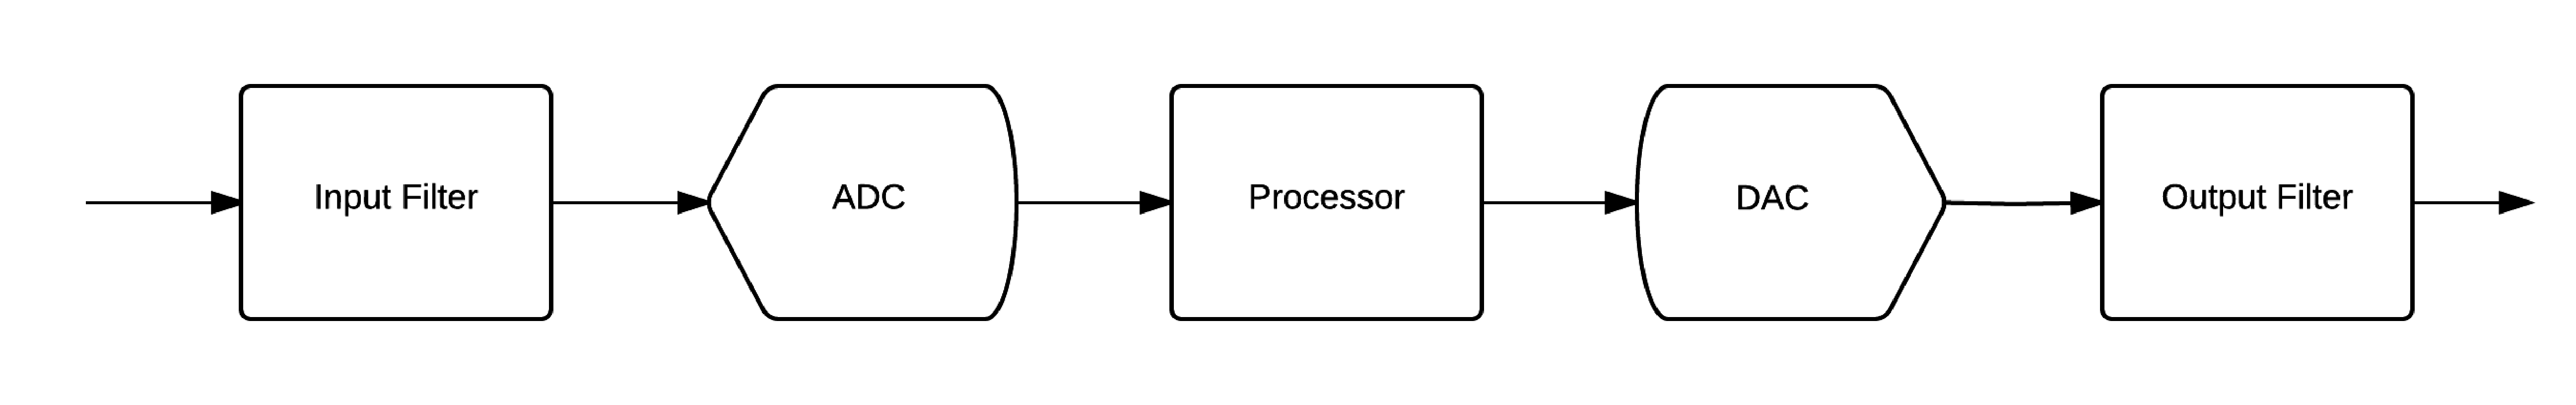
\includegraphics[width=0.8\textwidth]{./figures/sdr_basic_arch}
     \caption{ Software Defined Radio Basic Architecture
     \label{fig:sdr_basic}}
 \end{figure}


Implementations may vary a lot, some common implementations are Made in matlab
through Simulink and use the computer’s video card as a medium of communication.
A more difficult but more interesting implementation involves the use of DSP chips
to implement the signal processing functions and some cheap ADC and DAC chips can
compose the SDR system.\\

The most commercial and famous implementation of SDR is Gnuradio+USRP, USRP
stands for Universal Software Radio Peripheral \cite{web:usrp} and Gnuradio \cite{web:gnuradio}
is a software for PC which has various digital signal processing functions and
modulation schemes and comes with a driver to use USRP. The USRP itself is
basically and FPGA hooked with a transceiver, so this pair is broadly used in
research and academic environments.\\

When we talk about research and development of real-world systems there is always
a tradeoff or bottleneck, in SDR the bottleneck is the hardware related to the
antenna interface, the antenna is designed to work better in a specific bandwidth,
this can limit the application, of course this is only one example of bottleneck,
there are others like Oscillator frequency, PLL, and processor capability.\\


This work has a SDR like implementation done in FPGA and using the transceiver
AD9361 which makes baseband upconversion (Transmitter) and downconversion (Receiver),
filters and make analog to digital conversion and digital to analog conversion,
thus it is possible to implement transmitter and receiver with only one board,
however the most complex part does not lie in the system itself because some electronic
parts became a commodity, the complexity is in the modulation/demodulation blocks
and all the synchronization process, such topics shall be discussed in the chapter \ref{cap:digitalcomm}.
